A designed system must be tested to determine its effectiveness in solving the intended problem. This section presents the testing methodology used to assess the FPGA-based intrusion detection system described in Section~\ref{sec:Design_and_Development}, followed by an analysis of its performance under a range of traffic conditions and attack scenarios.
\subsection{Testing}
The FPGA-based intrusion detection system was tested to determine its
effectiveness in identifying malicious network activity using both controlled
and real-world conditions. The testing mainly focuses on two main aspects,
per-packet classification accuracy and sliding window based attack detection.

Datasets were constructed from real world PCAP (packet capture) files and then
converted into a hex-based format suitable for FPGA-based testing. The packets
in their original states are usable with a slight tweak to the verilog code
however a hex based format was due to memnory constraints in the FPGA. Each
dataset represents a specific attack type, allowing controlled evaluation of
detection performance. The following sections present the methodology and
results for each traffic type individually, followed by an analysis of overall
system behaviour.

\subsubsection{Packet Representation for a FPGA system}
The initial system design intended to use the onboard Ethernet (RJ45) interface
to enable real time packet capture and processing. However, implementation of
this approach required access to a licensed Ethernet axi IP core, which was not
available within the constraints of this project.

As a result, an alternative approach was used in which packet traces were pre
recorded and replayed from on-chip memory (BRAM). This approach provided a
repeatable method for evaluating the IDS, allowing testing across multiple
traffic scenarios taken from real-world datasets and synthetic dataets
generated for testing purposes.

While the original packets remained usable in their PCAP-derived form and
could, have been processed directly by the FPGA with minor modifications to the
parsing logic. However, doing so would require more exhaustive byte level
parsing and additional buffering within the hardware. This would not have been
feasible given the fact that the VC707 platform provides approximately 37,080
Kb Mb ($37080Kb \div 8 \approx 4.6 $MB) of on chip BRAM, as seen on page 7 of
the 7 Series FPGAs Data Sheet: Overview~\cite{noauthor_7_2020}. While this is
enough for basic buffering and control logic, it is not sufficient to store
large packet traces directly, this memory must also support buffering and
control logic, the available capacity for packet storage is further reduced in
practice. which is why a reduced packet format and smaller datasets were used
during testing. Due to the memory limitations of the FPGA, the original PCAP
packet format (shown in Fig.~\ref{fig:packet_comparison}(a)) was converted into
a more memory efficient representation, which is shown in
Figure~\ref{fig:packet_comparison}(b) below.

\begin{figure}[H]
    \centering

    \begin{minipage}{0.48\linewidth}
        \centering
        
\includegraphics[width=\linewidth]{pcap_original_format.png}

        \vspace{2pt}
        (a) Original PCAP packet view
    \end{minipage}
    \hfill
    \begin{minipage}{0.48\linewidth}
        \centering
        \begin{lstlisting}[style=hexstyle]
static const packet_record_t
syn_packet_real_world[] = {
{
    .len_words = 15,
    .words = {
        0x90B11CA2,
        0xC0D370F3,
        ...
    }
}
};
    \end{lstlisting}

        \vspace{2pt}
        (b) Compact FPGA packet format
    \end{minipage}

    \caption{Comparison of packet representations. The original PCAP format contains full protocol information, while the compact format stores packets as fixed 32-bit words for FPGA replay.}
    \label{fig:packet_comparison}

\end{figure}

In standard IPv4 based communication, packets follow a structured format
consisting of multiple fields distributed across several bytes. As shown in
Fig.~\ref{fig:ipv4_tcp_headers}, the IPv4 header has a minimum size of 20
bytes, containing fields such as source and destination IP addresses and
protocol identifiers.

\begin{figure}[H]
    \centering
    
\includegraphics[width=0.6\textwidth]{TCP_Header.png}
    \caption{A Typical IPv4 TCP header}
    \label{fig:ipv4_tcp_headers}
\end{figure}

While this structure is well suited for general-purpose networking, direct
processing of full PCAP byte streams on the FPGA was not adopted in this
implementation due to the aforementioned memory constraints. As mentioned
previously, the original system design intended to use the onboard Ethernet
interface for real-time packet capture and parsing, allowing packets to be
processed as they arrive rather than stored in BRAM, and therefore avoiding the
associated memory constraints.

To enable better/more testing, packets were transformed into a hex
representation in which the fields required for detection were kept and turned
into fixed 32-bit words. Key parts of the packet such as EtherType, IP
protocol, destination IP address, and TCP flags were encoded directly into
predefined positions within each word. In a conventional network, these fields
would be extracted by the Ethernet MAC and higher level protocol parsing logic.
In this implementation the extraction step is considered already performed,
allowing the FPGA to focus on the necesary fields.

\subsubsection{Packet Dataset and Test Setup}

To evaluate the performance of the FPGA-based intrusion detection system,
network traffic datasets were obtained from publicly available intrusion
detection benchmarks, specifically the CICIDS2017 and CICIDS2019 datasets.
These datasets provide realistic network traffic containing both innocuous
activity and also a number of attack behaviours.

Different subsets of the datasets were used to isolate specific traffic types
for controlled testing. ICMP and UDP traffic were extracted from the CICIDS2019
Friday Working Hours capture, which contains a mixturse of normal background
traffic and network activity representative of real-world conditions. TCP SYN
packets and normal traffic were extracted from the CICIDS2017 dataset, allowing
evaluation of connection based attacks such as SYN flooding then packets from
both datasets were combined to create a file with multiple attack patterns.

The packet captures were processed using \texttt{tshark} and \texttt{tcpdump}
to filter relevant traffic types. Custom Python scripts were then used to
convert the filtered packet data into a hardware-compatible format. Each packet
was represented as a sequence of 32-bit words and stored in header files,
ensuring the playing of the packets through the FPGA.

For consistency across experiments, each dataset was reduced to a fixed size of
64 packets. This ensures repeatability and allows direct comparison between
different traffic types and attack scenarios.

Example packets from the dataset are shown in Fig.~\ref{fig:packet_examples}.
These illustrate the structure of the packet data used for classification. In
particular, the TCP SYN packet (right) is characterised by the SYN flag (0x02),
which is used by the IDS to identify connection initiation behaviour and detect
potential SYN-based attacks.

\begin{figure}[H]
    \centering
    
\includegraphics[width=0.45\linewidth]{HeaderProtocolSRC_DST-Packet-1.jpg}
    \hfill
    
\includegraphics[width=0.45\linewidth]{SYN-Packet.jpg}

    \caption{Example packets used in testing. Left: normal TCP traffic. Right: TCP SYN packet, showing the SYN flag used for attack detection.}
    \label{fig:packet_examples}

\end{figure}

Each packet in the dataset is associated with a known classification, including
protocol type (TCP, UDP, ICMP) and, where applicable, specific flag
combinations (e.g. SYN, NULL, XMAS). This enables direct comparison between
expected classifications and the outputs produced by the IDS.

In addition to real-world datasets, synthetic attack traffic was generated
using the Nmap (Network Mapper) tool to provide controlled examples of specific
scan types. Nmap is a widely used network scanning tool that can make and
transmit packets with custom TCP flag combinations, which makes it suitable for
simulating attack behaviour.

Using Nmap, NULL and XMAS scan traffic were generated, a NULL scan, is where no
TCP flags are set, was generated using the command:

\begin{verbatim}
sudo nmap -sN -Pn <target-ip>
\end{verbatim}

An XMAS scan, which is where the FIN, PSH, and URG flags being set, was
generated using:

\begin{verbatim}
sudo nmap -sX -Pn <target-ip>
\end{verbatim}

Testing was carried out by replaying pre-processed packet datasets through the
FPGA-based IDS. Packets were read from BRAM and transmitted sequentially into
the processing pipeline, with the rate of packets being controlled using a
delay between packet injections.

The system performs both per-packet classification and sliding window-based
analysis. Individual packets are first classified based on protocol and flag
information, after which traffic is aggregated within a fixed time window to
identify higher-level behaviours such as flooding and volumetric attacks.

The following metrics were recorded during testing:

\begin{itemize}
    \item Total number of packets processed
    \item Protocol and flag-based classification results
    \item Detection of attack types (e.g. SYN flood, ICMP flood, volumetric attack)
    \item Number of packets observed within each detection window
\end{itemize}

These metrics allow evaluation of both the correctness of packet classification
and the behaviour of the sliding window detection mechanism under different
traffic rates and threshold configurations.
\subsection{Results}
\subsubsection{Threshold and Packet Rate Analysis}

The intrusion detection system uses a time-based sliding window to detect
high-volume traffic patterns. Two thresholds are defined: a volumetric
threshold, which triggers when the total number of packets within a window
exceeds a set value, and a flood threshold, which applies to protocol-specific
traffic such as TCP SYN packets.

In the code, the thresholds were defined as:

\begin{verbatim}
uint16_t vol_threshold = 15;
uint16_t flood_threshold = 11;
\end{verbatim}

Packet transmission rate is controlled by the delay between packet injections
from BRAM, implemented using the \texttt{usleep()} function in the main
program. This directly affects the number of packets that fall within each
detection window. Three different rates were evaluated:

\begin{itemize}
    \item \texttt{usleep(5000)} - increased packet rate
    \item \texttt{usleep(10000)} - base rate
    \item \texttt{usleep(20000)} - reduced packet rate
\end{itemize}

The test was performed using a dataset of normal network traffic taken from the
CICIDS2019 dataset. This dataset provides realistic background traffic without
significant attack patterns, making it suitable for analysing the effect of
packet rate and threshold selection on false flags.

\begin{table}[H]
    \centering
    \caption{Effect of packet transmission delay on volumetric detection}
    \begin{tabularx}{\linewidth}{|c|c|c|X|}
        \hline
        \textbf{Delay} & \textbf{Packets/window} & \textbf{Threshold} & \textbf{Detection result}          \\
        \hline
        usleep(5000)   & 21, 43                  & Yes                & Volumetric attack detected         \\
        \hline
        usleep(10000)  & 12, 23, 22              & Yes                & Attack detected in Windows 2 and 3 \\
        \hline
        usleep(20000)  & 5, 11, 12, 12, 12, 12   & No                 & No volumetric attack detected      \\
        \hline
    \end{tabularx}
    \label{tab:packet_rate_results}
\end{table}

\subsubsection{High Packet Rate: \texttt{usleep(5000)}}
At a higher packet rate, a greater number of packets are processed within each
250 ms detection window, as shown in Table~\ref{tab:packet_rate_results}.

In this configuration, the packet count in every window exceeded the volumetric
threshold, resulting in the detection of a volumetric attack. For example,
window counts of 21 and 43 packets were observed, both well above the threshold
of 15.

This shows that increasing the packet rate causes traffic to be concentrated
within fewer windows, increasing the likelihood of threshold-based detection
being triggered.

\subsubsection{Baseline Packet Rate: \texttt{usleep(10000)}}
At the baseline packet rate, packets are injected at a rate used in the other tests below,
resulting in a more balanced distribution across detection windows when compared
to the high and low packet rate configurations. The observed results are shown
in Table~\ref{tab:packet_rate_results}.

In this configuration, the number of packets per window was observed to be 12,
23, and 22. The first window remained below the volumetric threshold of 20,
while the second and third windows exceeded it. As a result, volumetric attack
detection was triggered as it only needs to be in one window to trigger an
attack.

This behaviour shows that the baseline rate lies close to the effective
detection boundary. Unlike the high packet rate case, where all windows exceed
the threshold, and the low packet rate case, where none do, the baseline rate
produces mixed results. This demonstrates that small variations in packet
timing can determine whether a threshold is crossed within a given window.

It is also worth noting that the total number of packets processed remains
approximately constant across the different configurations, as the same dataset
is replayed in each case. For the high and low packet rate tests, a total of 64
packets were observed, while the baseline configuration resulted in a slightly
lower total of 57 packets within the analysed windows.

This discrepancy is attributed to the interaction between packet timing and the
fixed window duration. At the baseline rate, some packets fall outside the
measured window boundaries due to timing alignment, resulting in a lower
observed total. This further illustrates the sensitivity of the system to
packet timing, where even small changes in inter-packet delay can influence how
traffic is distributed across detection windows.

\subsubsection{Low Packet Rate: \texttt{usleep(20000)}}
At a reduced packet rate, fewer packets are processed within each detection
window, as shown in Table.~\ref{tab:packet_rate_results}.

In this case, packet counts per window ranged between 5 and 12, remaining below
the volumetric threshold of 15. As a result, no volumetric attacks were
detected, despite the same total number of packets being transmitted.

This highlights the sensitivity of the detection mechanism to packet timing.
Although the overall traffic volume is unchanged, distributing packets over a
longer period reduces the likelihood of exceeding the detection threshold
within any given window.

\subsubsection{Discussion}
These results demonstrate that the detection system is strongly influenced by
packet arrival rate relative to the window size. Higher packet rates
concentrate traffic within a single window, increasing the likelihood of
triggering threshold-based alerts, while lower rates distribute traffic across
multiple windows, potentially avoiding detection.

This behaviour is expected for a sliding window-based detection mechanism and
illustrates the importance of selecting appropriate threshold values and window
sizes based on expected network traffic characteristics.

\subsubsection{Syn Flood}

\begin{table}[H]
    \centering
    \caption{Comparison of SYN flood detection for different SYN dataset sizes}
    \resizebox{\linewidth}{!}{
        \begin{tabular}{|c|c|c|c|}
            \hline
            \textbf{SYN Dataset Size} & \textbf{Observed packets per window} & \textbf{Detected attacks}                       & \textbf{Notes}                                            \\
            \hline
            64 packets                & 14, 23, 23, 4                        & SYN Flood; Volumetric Attack in Windows 2 and 3 & Larger dataset; dynamic target tracking disabled          \\
            \hline
            23 packets                & 14, 9                                & SYN Flood in Window 1 only                      & Reduced dataset; destination IP extracted as 192.168.50.4 \\
            \hline
        \end{tabular}
    }
    \label{tab:syn_results}
\end{table}

The results obtained from the SYN packet dataset (Taken from CCSID 2019) show that the system is
able to successfully identify SYN-based attack behaviour using both per-packet
classification and sliding window analysis. Two configurations were evaluated,
as shown in Table~\ref{tab:syn_results}, a reduced dataset and a larger
subset of the same dataset.

In the reduced configuration, a SYN flood was detected in the first window,
where 14 packets were observed, exceeding the flood threshold of 11. Following
windows contained fewer packets and did not trigger additional detections. In
contrast, when a larger subset of the dataset was evaluated, multiple windows
exceeded both the flood and volumetric thresholds. For example, packet
counts of 23 per window resulted in simultaneous triggering of both SYN flood
and volumetric attack alerts.

This behaviour is expected, as a higher concentration of SYN packets within a
single detection window increases both the protocol-specific count and the
total packet volume, allowing both thresholds to be exceeded. In compatison, when
fewer packets are present within a window, only some windows may exceed the SYN
flood threshold, and the volumetric threshold is less likely to be triggered.

Further analysis of the dataset, shown in Fig.~\ref{fig:syn_ports}, shows
that the majority of SYN packets are directed towards a single destination IP
address across multiple ports. This pattern is characteristic of SYN-based
scanning or probing, where a host attempts to initiate connections across a
range of ports. This behaviour is also reflected in the target tracking results, where only a
single dynamic destination IP was identified. Although additional destination
IPs are present within the dataset, they are associated with a small
number of packets and do not trigger the detection
window. As a result, only the main target exceeds the relevant thresholds
and is recorded by the system. The observed traffic behaviour aligns with the IDS output, where repeated SYN
packets within a short time interval result in the flood threshold being
exceeded.

Overall, these results show that the detection system is sensitive to
both traffic composition and the number of packets present within each
detection window. The same underlying traffic can produce different detection
outcomes depending on how packets are distributed across the fixed detection
windows.


\begin{figure}[H]
    \centering
    
\includegraphics[width=0.8\linewidth]{SYN_32_targets_proof_dynamic_memory.png}
    \caption{Extracted destination ports from the SYN packet dataset using \texttt{tcpdump}. The repeated destination IP with varying ports indicates SYN-based scanning or probing behaviour.}
    \label{fig:syn_ports}
\end{figure}

\subsubsection{Mixed Packets}
To further test the behaviour of the IDS under more realistic conditions, a
mixed traffic scenario was made combining both attack and non-attack
vectors. The generated scenario, shown in
Fig.~\ref{fig:mixed_topology}, is made up of of multiple hosts communicating through
a central switch, with both normal traffic and attack traffic directed towards
selected targets.

\begin{figure}[H]
    \centering
    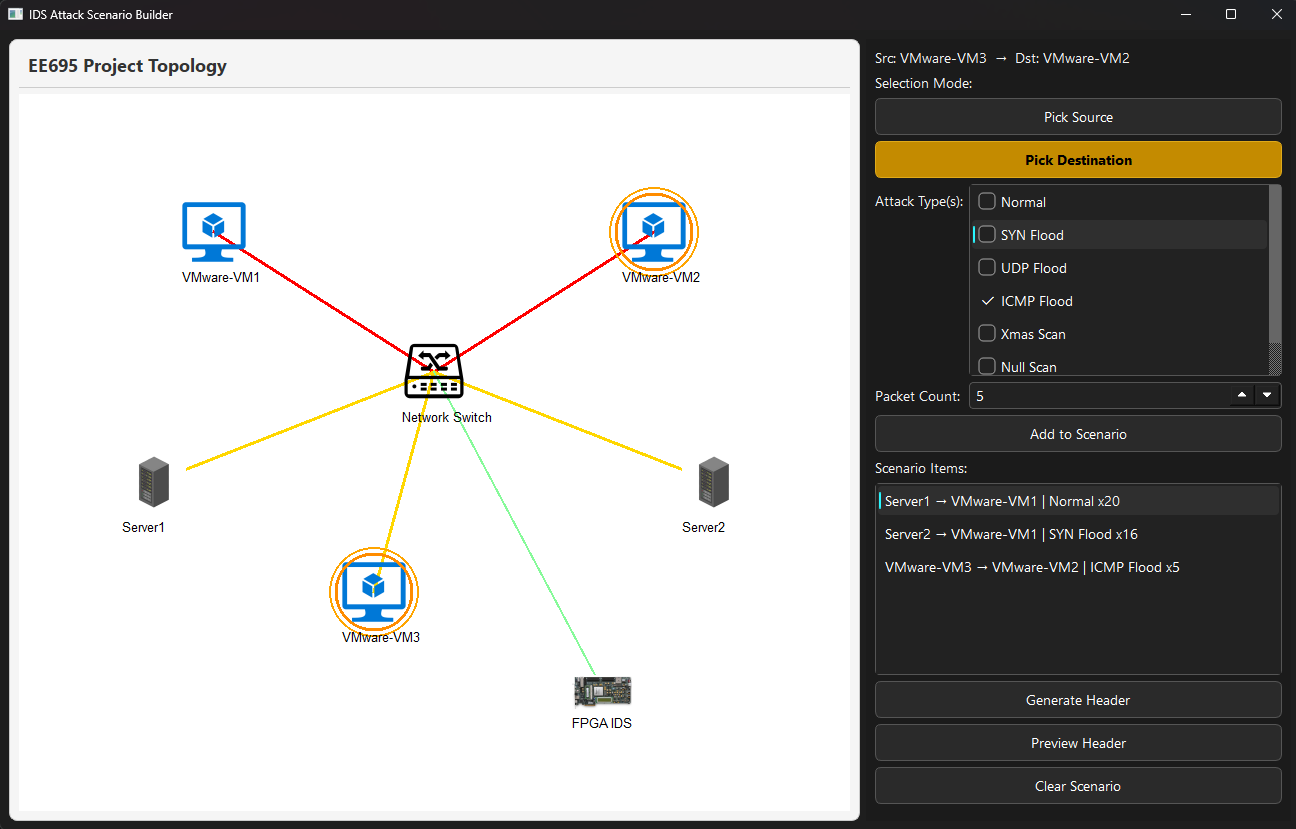
\includegraphics[width=0.8\linewidth]{Images/mixed_packets_scenario.png}
    \caption{Mixed traffic scenario generated using the IDS attack scenario builder}
    \label{fig:mixed_topology}
\end{figure}

In this test, three traffic sources and two destinations were defined. Server1 generated 20
normal packets directed towards VMware-VM1, representing a non attack vector. Then Server2 generated 16 TCP SYN packets towards the same destination, simulating a SYN flood attack. Additionally, VMware-VM3 generated a
5 ICMP packets directed towards VMware-VM2. It is worth noting that the source/destinatons were defined as:

\begin{table}[H]
    \centering
    \caption{Network Node Configuration}
    \begin{tabular}{ll}
        \toprule
        \textbf{Node Name} & \textbf{IP Address}     \\
        \midrule
        Network Switch     & \texttt{192.168.10.1}   \\
        VMware-VM1         & \texttt{192.168.10.3}   \\
        VMware-VM2         & \texttt{192.168.10.4}   \\
        Server1            & \texttt{192.168.10.5}   \\
        Server2            & \texttt{192.168.10.6}   \\
        VMware-VM3         & \texttt{192.168.10.7}   \\
        FPGA IDS           & \texttt{192.168.10.100} \\
        \bottomrule
    \end{tabular}
\end{table}

This results in a total of 41 packets, with the majority of traffic concentrated on a
single target. The results of this experiment are shown in
Fig.~\ref{fig:mixed_results}, which is the serial monitor output coming from the FPGA. Packets were distributed across four detection windows, with counts of 5, 12, 12, and 12 packets respectively, which add up to the expected 41 packets. Three of these windows exceeded the volumetric threshold of 10 packets, and
therefore a volumetric alert was triggered.

\begin{figure}[H]
    \centering
    
\includegraphics[width=0.875\linewidth]{images/proof_multiple_packets.png}
    \caption{Window-level output for mixed traffic scenario}
    \label{fig:mixed_results}
\end{figure}

As we can see the IDS successfully identified a SYN flood targeting VMware-VM1. As shown in the final output, a
total of 16 SYN packets were reported, exceeding the configured
flood threshold and it also means the IDS system recorded all packets, as seen in Fig~\ref{fig:mixed_topology} there was 16 SYN packets generated.

In contrast, no alerts were generated for VMware-VM2. Although ICMP traffic was
present, only 5 packets were observed, which remains well below the configured
flood threshold. As a result, this traffic was correctly classified as
non-malicious.

It is also noted that no dynamic targets were detected during this experiment.
All observed destination IP addresses correspond to predefined hosts within the
system, and therefore no additional target entries were created. This confirms
that the dynamic target mechanism operates only on previously unseen
destinations.

These results show that the IDS is capable of distinguishing between
benign and malicious traffic within a mixed dataset, while also correctly
associating detected attacks with specific targets. The system is able to detect
protocol-specific attacks such as SYN floods even when packet arrivals are
distributed across multiple detection windows, preventing individual windows
from exceeding volumetric thresholds.

This behaviour shows the importance of combining per-packet classification
with sliding window implementation. Sliding window analysis is effective for identifying short bursts of high traffic, whereas per-target statistics allow detection of attacks that are spread over time. This is important in mixed traffic scenarios, where malicious packets may be interwoven with normal traffic.

\subsubsection{ICMP Flood}

\begin{table}[H]
    \centering
    \caption{ICMP flood detection results using CICIDS2017 dataset}
    \resizebox{\linewidth}{!}{
        \begin{tabular}{|c|c|c|c|}
            \hline
            \textbf{Window} & \textbf{Packets in window} & \textbf{Detected attacks} & \textbf{Notes}               \\
            \hline
            Window 1        &    3 & None                          & Below all thresholds         \\
            \hline
            Window 2        & 23    & ICMP Flood; Volumetric Attack & Exceeds both thresholds      \\
            \hline
            Window 3        & 24    & ICMP Flood; Volumetric Attack & Sustained high packet rate   \\
            \hline
            Window 4        & 14    & ICMP Flood                    & Exceeds flood threshold only \\
            \hline
        \end{tabular}
    }
    \label{tab:icmp_results}
\end{table}

The ICMP flood detection capability of the system was tested using a dataset
taken from the CICIDS2017 traffic capture. The results, as summarised in
Table~\ref{tab:icmp_results}, show that the IDS is able to correctly
identify ICMP-based attack behaviour.

In this experiment, packets were distributed across four detection windows
containing 3, 23, 24, and 14 packets respectively. The first window remained
below both the volumetric threshold of 15 and the flood threshold of 11, and
therefore did not trigger any alerts. In contrast, the second and third windows
exceeded both thresholds, resulting in simultaneous detection of ICMP flood and
volumetric attacks.

The fourth window contained 14 packets, which is below the volumetric threshold
but above the ICMP flood threshold. As a result, only the ICMP flood alert was
triggered. This demonstrates that the system can distinguish between
protocol-specific flooding behaviour and overall traffic volume, even when the
two conditions do not occur simultaneously.

The final attack summary showed that all traffic was directed towards a single
target, VMware-VM1 (192.168.10.3), with a total of 62 ICMP packets observed.
This exceeds both the flood and volumetric thresholds when considered over the
entire capture, resulting in both alerts being reported at the target level.

It should be noted that the IP address observed in this experiment originates
from the real-world CICIDS2017 dataset. In this case, the destination address
coincidentally matches one of the predefined IPs used within the test topology
(192.168.10.3). As a result, the traffic is labelled as VMware-VM1 within the
system, although it does not necessarily correspond to the same physical host.

These results confirm that the ICMP detection logic operates correctly on
real-world traffic. Similar to the SYN flood case, detection is influenced by
how packets are distributed across detection windows. High concentrations of
packets within a single window result in both flood and volumetric alerts,
whereas lower concentrations may only trigger protocol-specific detection.

Overall, this experiment shows that the IDS is capable of reliably
detecting ICMP flood behaviour and correctly attributing it to the relevant
target, even when traffic is distributed across multiple detection windows.


\subsubsection{NULL Scan Detection}

\begin{table}[H]
    \centering
    \caption{NULL scan detection results using CICIDS2017 dataset}
    \resizebox{\linewidth}{!}{
        \begin{tabular}{|c|c|c|c|}
            \hline
            \textbf{Window} & \textbf{Packets in window} & \textbf{Detected attacks}    & \textbf{Notes}             \\
            \hline
            Window 1        & 1 & None                         & Single packet              \\
            \hline
            Window 2        & 24    & NULL Scan; Volumetric Attack & Exceeds both thresholds    \\
            \hline
            Window 3        & 23    & NULL Scan; Volumetric Attack & Sustained high packet rate \\
            \hline
            Window 4        & 16    & NULL Scan; Volumetric Attack & Above both thresholds      \\
            \hline
        \end{tabular}
    }
    \label{tab:null_results}
\end{table}

The NULL scan detection ability of the IDS was tested using a dataset
derived from the CICIDS2017 traffic capture. A NULL scan is a TCP-based probing
technique in which packets are transmitted with all control flags unset. Under
normal TCP operation, at least one flag is expected, and therefore packets with
no flags set are considered anomalous and indicative of scanning activity.

The results, summarised in Table~\ref{tab:null_results}, demonstrate that the
system is able to correctly identify NULL scan behaviour using both per-packet
classification and sliding window analysis.

In this experiment, packets were distributed across four detection windows
containing 1, 24, 23, and 16 packets respectively. The first window contained
only a single packet and therefore remained below the volumetric threshold of
15. However, a NULL scan alert was still triggered due to the presence of a
packet with no TCP flags set, confirming that the per-packet classification
logic is functioning correctly.

The remaining windows contained significantly higher packet counts, exceeding
both the flood threshold of 11 and the volumetric threshold of 15. As a result,
both NULL scan and volumetric attack alerts were triggered. This demonstrates
that the system is capable of identifying both protocol-specific anomalies and
high-volume traffic conditions within the same detection framework.

It is noted that no entries were produced in the final ``Attacks Detected''
section. This behaviour differs from previous experiments and is due to the
software-based aggregation stage, which relies on consistent extraction of
destination IP addresses. For this dataset, the destination information was not
reliably captured during readback, preventing packets from being grouped into
per-target statistics.

However, the window summary is generated directly by the FPGA and reflects
real-time detection based on packet activity within each detection window. The
correct identification of NULL scan behaviour across multiple windows therefore
confirms that the hardware detection logic is operating as intended.

Overall, these results demonstrate that NULL scan detection is correctly
implemented at the hardware level. While limitations in the software interface
affect per-target reporting, the core detection mechanisms remain robust and
capable of identifying anomalous TCP behaviour in real-world traffic.



\subsubsection{XMAS Scan Detection}

\begin{table}[H]
    \centering
    \caption{XMAS scan detection results}
    \resizebox{\linewidth}{!}{
        \begin{tabular}{|c|c|c|c|}
            \hline
            \textbf{Window} & \textbf{Packets in window} & \textbf{Detected attacks} & \textbf{Notes} \\
            \hline
            Window 1 & 18 & XMAS Scan; Volumetric Attack & Exceeds both thresholds \\
            \hline
            Window 2 & 23 & XMAS Scan; Volumetric Attack & Sustained high packet rate \\
            \hline
            Window 3 & 23 & XMAS Scan; Volumetric Attack & Consistent detection across windows \\
            \hline
        \end{tabular}
    }
    \label{tab:xmas_results}
\end{table}

The XMAS scan detection capability of the IDS was evaluated using a dataset
containing TCP packets with multiple control flags set. An XMAS scan is a type
of probing technique in which packets are transmitted with several TCP flags
enabled simultaneously (typically FIN, PSH, and URG), resulting in an unusual
combination of flags that is not normally observed during standard TCP
communication.

The results, summarised in Table~\ref{tab:xmas_results}, demonstrate that the
system is able to consistently identify XMAS scan behaviour across all
detection windows. In this experiment, packets were distributed across three
windows containing 18, 23, and 23 packets respectively.

In all cases, the number of packets exceeded both the flood threshold of 11 and
the volumetric threshold of 15. As a result, both XMAS scan and volumetric
attack alerts were triggered in each window. This indicates that the IDS is
able to reliably detect abnormal TCP flag combinations while also identifying
high-volume traffic patterns.

No entries were produced in the ``Attacks Detected'' section for this
experiment. As observed in the NULL scan case, this is attributed to the
software-based aggregation stage, which depends on consistent extraction of
destination IP addresses. For this dataset, destination information was not
reliably captured, preventing packets from being grouped into per-target
statistics.

Despite this limitation, the window-level results confirm that the FPGA-based
detection logic is functioning correctly. The consistent identification of XMAS
scan behaviour across all windows demonstrates that the system can accurately
detect this class of anomaly in real-time.

Overall, these results show that the IDS is capable of reliably detecting XMAS
scan activity using both per-packet classification and sliding window
analysis, even when target-level aggregation is not available.


\subsubsection{UDP Flood Detection}

\begin{table}[H]
    \centering
    \caption{UDP flood detection results}
    \resizebox{\linewidth}{!}{
        \begin{tabular}{|c|c|c|c|}
            \hline
            \textbf{Window} & \textbf{Packets in window} & \textbf{Detected attacks} & \textbf{Notes} \\
            \hline
            Window 1 & 18 & UDP Flood; Volumetric Attack & Exceeds both thresholds \\
            \hline
            Window 2 & 23 & UDP Flood; Volumetric Attack & Sustained high packet rate \\
            \hline
            Window 3 & 23 & UDP Flood; Volumetric Attack & Consistent detection across windows \\
            \hline
        \end{tabular}
    }
    \label{tab:udp_results}
\end{table}

The UDP flood detection capability of the IDS was evaluated using a dataset
containing a high volume of UDP packets directed towards a single destination.
A UDP flood is a type of denial-of-service attack in which a target is
overwhelmed with a large number of UDP packets, often causing resource
exhaustion due to the need to process or respond to each packet.

The results, summarised in Table~\ref{tab:udp_results}, demonstrate that the
system is able to correctly identify UDP flood behaviour across all detection
windows. In this experiment, packets were distributed across three windows
containing 18, 23, and 23 packets respectively.

In all cases, the number of packets exceeded both the flood threshold of 11 and
the volumetric threshold of 15. As a result, both UDP flood and volumetric
attack alerts were triggered in each window. This indicates that the IDS is
able to detect high-rate UDP traffic and correctly classify it as malicious
based on packet volume and protocol type.

No entries were produced in the ``Attacks Detected'' section for this
experiment. As observed in previous cases, this is attributed to the
software-based aggregation stage, which relies on consistent extraction of
destination IP addresses. For this dataset, the destination information was not
reliably captured, preventing packets from being grouped into per-target
statistics.

Despite this limitation, the window-level results confirm that the FPGA-based
detection logic is functioning correctly. The consistent identification of UDP
flood behaviour across all windows demonstrates that the system can accurately
detect high-volume UDP-based attacks in real time.

Overall, these results show that the IDS is capable of reliably detecting UDP
flood activity using both sliding window analysis and per-packet
classification, further validating the effectiveness of the system across
multiple protocol types.


\subsection{System Limitations}

While the proposed FPGA-based IDS demonstrates effective detection of multiple
attack types, several limitations were identified during implementation and
testing.

One key limitation is the reliance on on-chip BRAM for packet storage and
processing. As the available BRAM on the FPGA is limited, only a relatively
small number of packets can be buffered at any given time. This constrains the
size of datasets that can be replayed and necessitates the use of reduced or
compact packet representations. As observed during testing, larger datasets can
lead to instability or incomplete processing, particularly when additional
features such as dynamic target tracking are enabled.

Dynamic target tracking introduces further resource constraints. The allocation
of memory for storing per-target statistics consumes valuable BRAM resources,
which limits the number of concurrent targets that can be tracked. In this
implementation, the number of dynamic targets is therefore restricted, and in
some experiments this feature was disabled to ensure reliable system operation.
This highlights a trade-off between detection capability and hardware resource
usage.

Another limitation arises from the software-based aggregation stage. The final
``Attacks Detected'' summary depends on consistent and reliable extraction of
destination IP addresses from the hardware. As observed in the NULL and XMAS
scan experiments, unstable or inconsistent metadata readback can prevent
packets from being correctly grouped, resulting in missing per-target summaries
despite correct detection at the window level. This indicates that the
communication interface between hardware and software is a critical component
of the overall system reliability.

From a detection perspective, the IDS is primarily threshold-based and focuses
on a predefined set of attack signatures, including SYN floods, ICMP floods,
UDP floods, and TCP flag-based scans. While effective for these cases, this
approach may not generalise well to more complex or subtle attack patterns.
For example, attacks such as ACK floods or low-rate distributed attacks may not
be detected if they do not exceed the configured thresholds within a given
window. Similarly, the system does not perform deep packet inspection or
stateful flow analysis, limiting its ability to detect application-layer or
evasion-based attacks.

Finally, the use of fixed detection windows introduces sensitivity to packet
timing. As demonstrated in earlier experiments, the same traffic can produce
different detection outcomes depending on how packets are distributed across
windows. This can lead to borderline cases where attacks are inconsistently
detected, particularly when traffic rates are close to threshold values.

Overall, these limitations highlight the challenges of implementing an IDS on
resource-constrained hardware. While the system achieves efficient real-time
detection for a range of common attack types, further improvements in memory
management, metadata handling, and detection algorithms would be required to
support more complex and scalable network monitoring scenarios.




\subsection{Comparison with Software-Based IDS}

\begin{table}[H]
\centering
\caption{Comparison between FPGA-based IDS and software IDS}
\begin{tabular}{|c|c|c|}
\hline
\textbf{Feature} & \textbf{Software IDS (e.g. Snort)} & \textbf{FPGA IDS (This Work)} \\
\hline
Latency & High (ms) & Low (hardware-level) \\
\hline
Power Consumption & High & Low \\
\hline
Parallel Processing & Limited & Highly parallel \\
\hline
Flexibility & High & Moderate \\
\hline
\end{tabular}
\end{table}
